\RequirePackage{ifluatex}
\let\ifluatex\relax

\documentclass[aps,%
12pt,%
final,%
oneside,
onecolumn,%
musixtex, %
superscriptaddress,%
centertags]{article} %% 
\topmargin=-40pt
\textheight=650pt
\usepackage[english,russian]{babel}
\usepackage[utf8]{inputenc}
%всякие настройки по желанию%
\usepackage[colorlinks=true,linkcolor=blue,unicode=true]{hyperref}
\usepackage{euscript}
\usepackage{supertabular}
\usepackage[pdftex]{graphicx}
\usepackage{amsthm,amssymb, amsmath}
\usepackage{textcomp}
\usepackage[noend]{algorithmic}
\usepackage[ruled]{algorithm}
\selectlanguage{russian}

\begin{document}

\begin{titlepage} 
\begin{center}
% Upper part of the page
%\textbf{\Large САНКТ-ПЕТЕРБУРГСКИЙ ГОСУДАРСТВЕННЫЙ ЭКОНОМИЧЕСКИЙ УНИВЕРСИТЕТ} \\[1.0cm]
%\textbf{\large Кафедра Прикладной Математики и Информатики}\\[3.5cm]
 
% Title
\textbf{}\\[10.0cm]
\textbf{\LARGE Финансовая математика}\\[0.5cm]
\textbf{\Large ПМ-1701} \\[0.2cm]

%supervisor
\begin{center} \large
{Преподаватель:} \\[0.5cm]
\textsc {Чернов Алексей Викторович}\\
{alex\_tche@mail.ru}\\
\end{center}
% \begin{flushright} \large
%\emph{Рецензент:} \\
%д.ф. - м.н., профессор \textsc{Надеемся Нам Помогут}
%\end{flushright}
%\begin{flushright} \large
%\emph{Заведующий кафедрой:} \\
%д.ф. - м.н., профессор \textsc{Не Обмани Себя}
%\end{flushright}
\vfill 

% Bottom of the page
{\large {Санкт-Петербург}} \par
{\large {2020 г., 6 семестр}}
\end{center} 
\end{titlepage}

% Table of contents
\begin{thebibliography}{3}
	\bibitem{Sulsky1994}
	Sulsky D., Chen Z., Schreyer H. L.  A particle method for history-dependent materials // Computer Methods in Applied Mechanics and Engineering. --- 1994, V. 118. --- P. 179--196.
	\bibitem{LiuLiu}
	Liu G. R., Liu M. B. Smoothed particle hydrodynamics: a meshfree particle method. --- Singapore : World Scientific Publishing. --- 2003. --- 449 p.
\end{thebibliography}
\tableofcontents
\newpage
\section{Конспекты лекций}
\subsection{ Простая и сложная процентная ставка 05.02.2020} 

Для иллюстрации понимания работы сложного и простого процента введем следующие обозначения:
\begin{itemize} 
  \item $i$ - процентная ставка (по умолчанию годовая)
  \item $t$ - срок вклада
  \item $S_{0} = P$ - начальный вклад
  \item \textbf{$S$} - конечный вклад
  
\end{itemize}
\textbf{Def 1}: \textit{Простыми процентами} называются такие процентные ставки, которые применяются к одной и той же первоначальной сумме на протяжении всей финансовой операции \\
\textbf{Def 2}: \textit{Сложными процентами} называются ставки, применяемые после каждого интервала начисления к сумме первоначального долга и начисленных за предыдущие интервалы процентов.

\label{first_table}
\begin{table}[H]
	\begin{center}
	
		\begin{tabular}{c|c|c} 
		t (год) & Простой процент (\%) & Сложный процент (\%) \\ \hline
		0 & \textbf{100} & 100  \\ 
		1 & \textbf{110} & 110 \\ 
		2 & \textbf{120} & 121
		\end{tabular}
	\caption{Пример использования сложных и простых процентов}
	\end{center}
\end{table}
\begin{flushleft}
	Для простых процентов получаем следующие формулы:
\end{flushleft}

\begin{itemize} 
	\item Формула для $S_{n+1}$: $S_{n+1}=S_n+S_0\cdot i  $
	\item Формула для конечного вклада: $S=P+P\cdot i\cdot n=P\cdot (1+i\cdot n) $
	\item Формула для начального вклада: $P=\frac{S}{1+i\cdot n} $ 
	\item Формула для процентной ставки: $i=\frac{\frac{S}{P}-1}{t}=\frac{S-P}{t\cdot P}$
	\item Формула для продолжительности вклада: $ t=\frac{\frac{S}{P}-1}{i}=\frac{S-P}{i\cdot P}$
\end{itemize}
\begin{flushleft}
	Для сложных процентов получаем следующие формулы:
\end{flushleft}

\begin{itemize} 
	\item Формула для $S_{n+1}$: $S_{n+1}=S_n\cdot (1+i) = S_n + S_n\cdot i  $
	\item Формула для конечного вклада: $S = P\cdot (1+i)^n $
	\item Формула для начального вклада: $P=\frac{S}{(1+i)^n} $ 
	\item Формула для процентной ставки: $i=\sqrt[t]{\frac{S}{P}}-1$
	\item Формула для продолжительности вклада: $ t=log_{(1+i)} \frac{S}{P}$
\end{itemize}

\subsubsection{Срок удвоения вклада:}

\textbf {Для простого процента:} \\ [0.3cm]
$2P=P\cdot(1+i\cdot t_{new})$ \\ [0.3cm]
$t_{new}=\frac{1}{i}$ \\ [0.3cm]
\textbf {Для простого процента:} \\ [0.3cm]
$2P=P\cdot(1+i)^{t_{new}}$ \\ [0.3cm]
$2 = (1+i)^{t_{new}}$ \\ [0.3cm]
$t_{new}=log_{(1+i)} 2$ 

\begin{flushleft}
\subsubsection{Задача о.в Манхэттен:}
\end{flushleft}
\label{second_table}
\begin{table}[H]
	\begin{center}
	\caption{Данные о Манхэттене}
		\begin{tabular}{c|c} 
		t (год) & Деньги (\$) \\ \hline
		$t_1$ - 1626 год & $P - 24$ \\ \hline
		$t_2$ - 2019 год & $S - 49\cdot 10^9$
		\end{tabular}
	\end{center}
\end{table}
\begin{flushleft}
\textbf{Вопрос}: Какова процентная ставка при простом и сложном проценте?
\end{flushleft}
\textbf{Решение:} \\
Простой процент: \\[0.2cm]
$i=\frac{\frac{S}{P}-1}{t}=\frac{S-P}{(t_2-t_1)\cdot P}=\frac{49\cdot 10^9-24}{24*(2019-1626)}=5.19 \cdot 10^6$ \\[0.5cm]
Сложный процент: \\[0.2cm]
$i=\sqrt[(t_2-t_1)]{\frac{S}{P}}-1=\sqrt[2019-1626]{\frac{49\cdot 10^9}{24}}-1 = 0.056 = 5.6\%$ \\[0.5cm]
Срок удвоения оклада: \\[0.2cm]
$t_{new}=log_{(1+i)} 2 = log_{(1+0.056)} 2 = 12.7 \approx 13$ лет

\subsubsection{Смешанная ставка:}

\textbf{Def 3}: \textit{Смешанная процентная ставка} - ставка, которая осуществляется по следующему правилу - в пределах года используется простая ставка, а остальные - по сложной  \\[0.3cm]
Формула для смешанной процентной ставки: \\[0.3cm]
$S = P\cdot (1+i_c)^{[t]} + P\cdot (1+i_c)^{[t]} \cdot {\{t\}}\cdot i_p = P(1+i_c)^{[t]} \cdot (1 + {\{t\}}\cdot i_p ) $ \\ [0.3cm]
где ${[t]}$ - целая часть числа, а  ${\{t\}}$ - дробная.
%\begin{figure}[h!]
\begin{center}

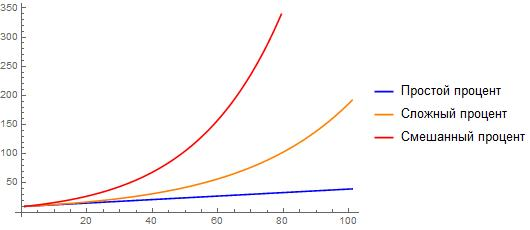
\includegraphics[scale=0.6]{images/first.jpg}

\end{center}
%\end{figure}

\subsection{09.02.2020}


\end{document}